\documentclass[11pt]{article}
\usepackage[margin=1in]{geometry}
\usepackage{enumitem}
\usepackage{hyperref}
\usepackage{graphicx}
\usepackage{array}
\usepackage{multicol}
\usepackage{longtable}
\usepackage{titlesec}
\usepackage{booktabs}
\usepackage{amsmath}
\usepackage{float}
\usepackage{sectsty}
\sectionfont{\fontsize{14}{16}\selectfont}
\subsectionfont{\fontsize{12}{14}\selectfont}


\begin{document}

\textbf{SVM - RBF Kernel}
\begin{verbatim}
svr_model = SVR(kernel='rbf', C=1, gamma='scale')
mae_list, mse_list, rmse_list, r2_list, all_actuals, all_predictions = [], [], [], 
    [], [], []

for fold, (train_index, val_index) in enumerate(kf.split(X), start=1):
    X_train, X_val = X.iloc[train_index], X.iloc[val_index]
    y_train, y_val = y.iloc[train_index], y.iloc[val_index]
    
    svr_model.fit(X_train, y_train)
    y_pred = svr_model.predict(X_val)

    all_actuals.extend(y_val)
    all_predictions.extend(y_pred)

    mae = mean_absolute_error(y_val, y_pred)
    mse = mean_squared_error(y_val, y_pred)
    rmse = np.sqrt(mse)
    r2 = r2_score(y_val, y_pred)

    mae_list.append(mae)
    mse_list.append(mse)
    rmse_list.append(rmse)
    r2_list.append(r2)

    print(f"Fold {fold} - MAE: {mae:.2f}, MSE: {mse:.2f}, 
    RMSE: {rmse:.2f}, R2: {r2:.4f}")

avg_mae = np.mean(mae_list)
avg_mse = np.mean(mse_list)
avg_rmse = np.mean(rmse_list)
avg_r2 = np.mean(r2_list)

\end{verbatim}

\begin{figure}[H]
\centering
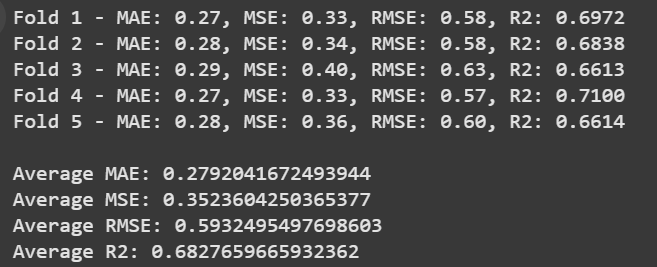
\includegraphics[width=0.9\textwidth]{expt2/rbfmetrics.png} 
\end{figure}

\begin{figure}[H]
\centering
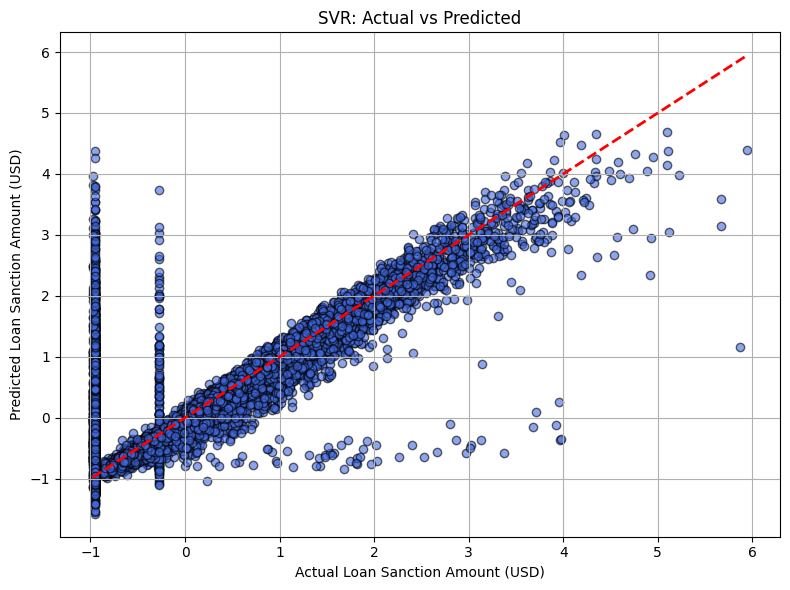
\includegraphics[width=0.8\textwidth]{expt2/rbfg1.png} 
\end{figure}

\begin{figure}[H]
\centering
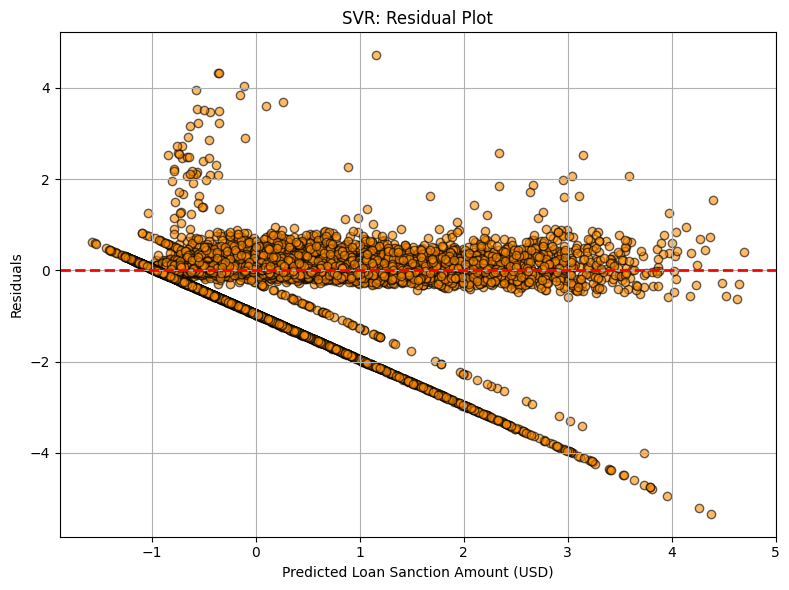
\includegraphics[width=0.8\textwidth]{expt2/rbfg2.png} 
\end{figure}

\vspace{1.7cm}
\textbf{SVM - Polynomial Kernel}
\begin{verbatim}
svr_model = SVR(kernel='poly', C=1, gamma='scale')
mae_list, mse_list, rmse_list, r2_list, all_actuals, all_predictions = [], [], [],
[], [], []
for fold, (train_index, val_index) in enumerate(kf.split(X), start=1):
    X_train, X_val = X.iloc[train_index], X.iloc[val_index]
    y_train, y_val = y.iloc[train_index], y.iloc[val_index]

    svr_model.fit(X_train, y_train)
    y_pred = svr_model.predict(X_val)

    all_actuals.extend(y_val)
    all_predictions.extend(y_pred)

    mae = mean_absolute_error(y_val, y_pred)
    mse = mean_squared_error(y_val, y_pred)
    rmse = np.sqrt(mse)
    r2 = r2_score(y_val, y_pred)

    mae_list.append(mae)
    mse_list.append(mse)
    rmse_list.append(rmse)
    r2_list.append(r2)

    print(f"Fold {fold} - MAE: {mae:.2f}, MSE: {mse:.2f}, 
    RMSE: {rmse:.2f}, R2: {r2:.4f}")

avg_mae = np.mean(mae_list)
avg_mse = np.mean(mse_list)
avg_rmse = np.mean(rmse_list)
avg_r2 = np.mean(r2_list)
\end{verbatim}

\begin{figure}[H]
\centering
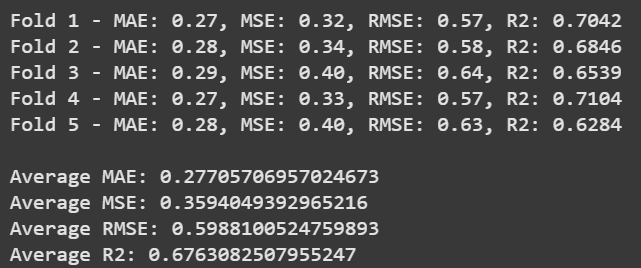
\includegraphics[width=0.9\textwidth]{expt2/polymetrics.png} 
\end{figure}

\begin{figure}[H]
\centering
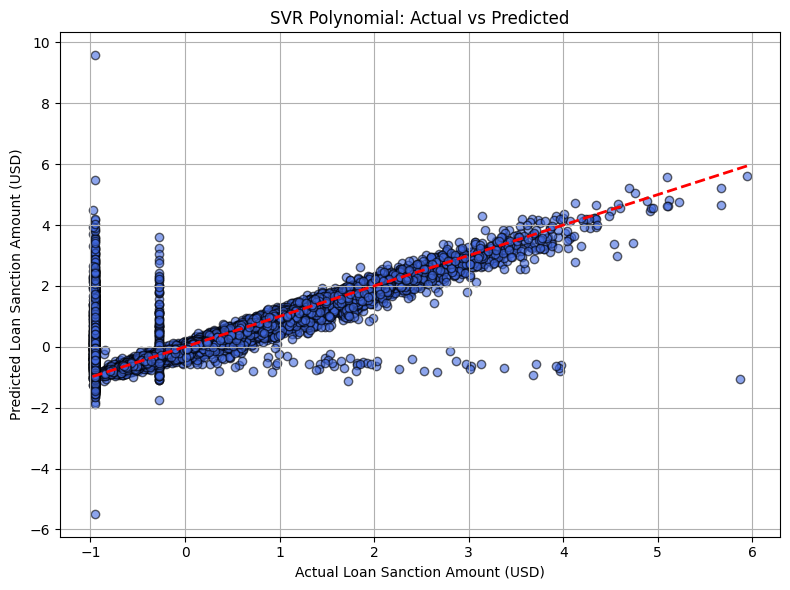
\includegraphics[width=0.8\textwidth]{expt2/polyg1.png} 
\end{figure}

\begin{figure}[H]
\centering
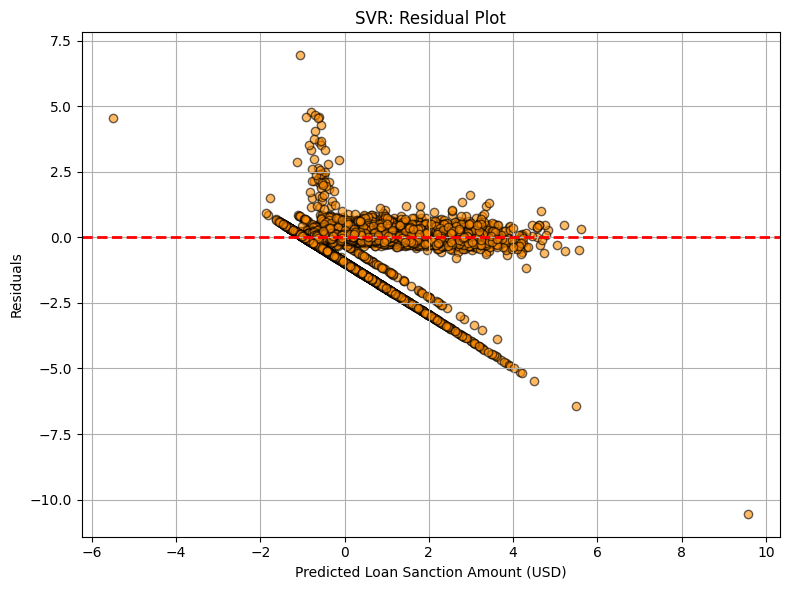
\includegraphics[width=0.8\textwidth]{expt2/polyg2.png} 
\end{figure}

\vspace{1.7cm}
\textbf{SVM - Linear Kernel}
\begin{verbatim}
svr_model = SVR(kernel='linear', C=1, gamma='scale')
mae_list, mse_list, rmse_list, r2_list, all_actuals, all_predictions = [], [], [],
[], [], []
for fold, (train_index, val_index) in enumerate(kf.split(X), start=1):
    X_train, X_val = X.iloc[train_index], X.iloc[val_index]
    y_train, y_val = y.iloc[train_index], y.iloc[val_index]

    svr_model.fit(X_train, y_train)
    y_pred = svr_model.predict(X_val)

    all_actuals.extend(y_val)
    all_predictions.extend(y_pred)

    mae = mean_absolute_error(y_val, y_pred)
    mse = mean_squared_error(y_val, y_pred)
    rmse = np.sqrt(mse)
    r2 = r2_score(y_val, y_pred)

    mae_list.append(mae)
    mse_list.append(mse)
    rmse_list.append(rmse)
    r2_list.append(r2)

    print(f"Fold {fold} - MAE: {mae:.2f}, MSE: {mse:.2f}, 
    RMSE: {rmse:.2f}, R2: {r2:.4f}")

avg_mae = np.mean(mae_list)
avg_mse = np.mean(mse_list)
avg_rmse = np.mean(rmse_list)
avg_r2 = np.mean(r2_list)
\end{verbatim}

\begin{figure}[H]
\centering
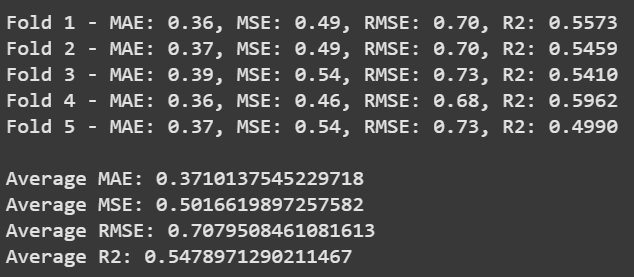
\includegraphics[width=0.9\textwidth]{expt2/linearmetrics.png} 
\end{figure}

\begin{figure}[H]
\centering
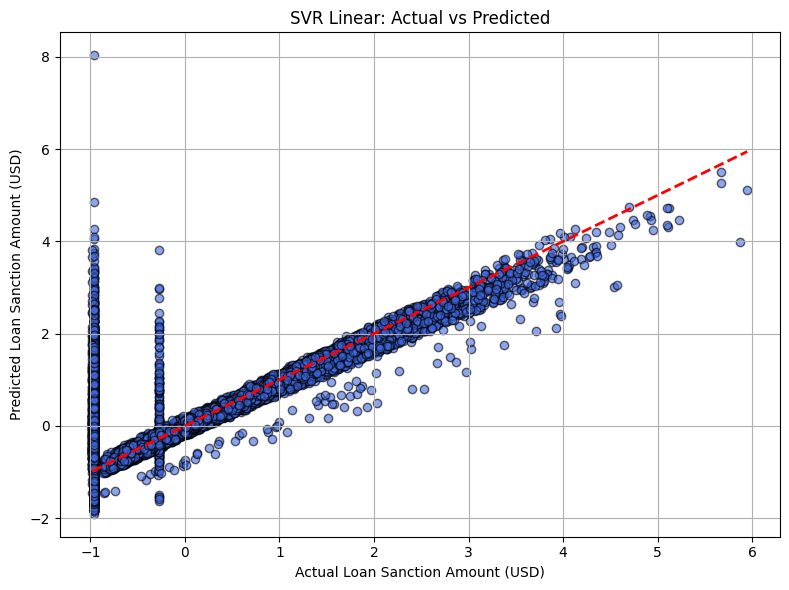
\includegraphics[width=0.8\textwidth]{expt2/linearg1.png} 
\end{figure}

\begin{figure}[H]
\centering
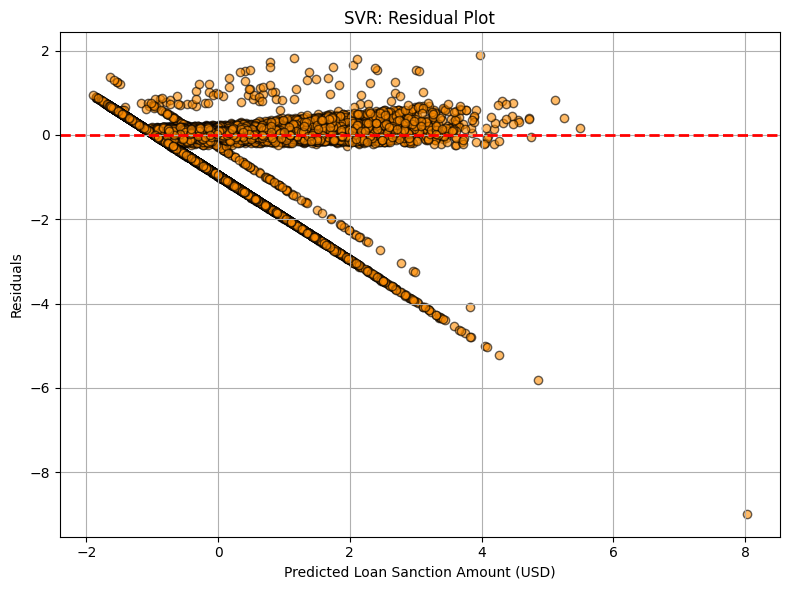
\includegraphics[width=0.8\textwidth]{expt2/linearg2.png} 
\end{figure}

\end{document}